%@+leo-ver=4-thin
%@+node:paoluzzi.20131121082536.1674:@shadow ../Documents/dev/test/larcc/src/tex/lar2psm.tex
%@+others
%@+node:paoluzzi.20131121082536.1675:larcc template
%@@language latex

\documentclass[11pt,oneside]{article}	%use"amsart"insteadof"article"forAMSLaTeXformat
\usepackage{geometry}		%Seegeometry.pdftolearnthelayoutoptions.Therearelots.
\geometry{letterpaper}		%...ora4paperora5paperor...
%\geometry{landscape}		%Activateforforrotatedpagegeometry
%\usepackage[parfill]{parskip}		%Activatetobeginparagraphswithanemptylineratherthananindent
\usepackage{graphicx}				%Usepdf,png,jpg,orepsßwithpdflatex;useepsinDVImode
								%TeXwillautomaticallyconverteps-->pdfinpdflatex		
\usepackage{amssymb,amsmath,amsthm}
\newtheorem{definition}{Definition}
\usepackage[colorlinks=true]{hyperref}

%----macros begin-----------------------------------------------------------------------------------
\usepackage{graphicx}
\usepackage{color}
\usepackage{amsthm}

%\renewenvironment{Shaded}{\pause\begin{snugshade}}{\end{snugshade}}
\def\twocolumns#1#2{\begin{columns}
\begin{column}{0.5\linewidth}#1\end{column}
\begin{column}{0.5\linewidth}#2\end{column}
\end{columns}}
\def\mytwocolumns#1#2#3#4{\begin{columns}
\begin{column}{#1\linewidth}#2\end{column}
\begin{column}{#3\linewidth}#4\end{column}
\end{columns}}
\def\mythreecolumns#1#2#3#4#5#6{\begin{columns}
\begin{column}{#1\linewidth}#2\end{column}
\begin{column}{#3\linewidth}#4\end{column}
\begin{column}{#5\linewidth}#6\end{column}
\end{columns}}
\def\threecolumns#1#2#3{\begin{columns}
\begin{column}{0.33\linewidth}#1\end{column}
\begin{column}{0.33\linewidth}#2\end{column}
\begin{column}{0.33\linewidth}#3\end{column}
\end{columns}}
\def\fourcolumns#1#2#3#4{\begin{columns}%
\begin{column}{0.25\linewidth}#1\end{column}%
\begin{column}{0.25\linewidth}#2\end{column}%
\begin{column}{0.25\linewidth}#3\end{column}%
\begin{column}{0.25\linewidth}#4\end{column}%
\end{columns}}

\def\conv{\mbox{\textrm{conv}\,}}
\def\aff{\mbox{\textrm{aff}\,}}
\def\E{\mathbb{E}}
\def\R{\mathbb{R}}
\def\Z{\mathbb{Z}}
\def\tex{\TeX}
\def\latex{\LaTeX}
\def\v#1{{\bf #1}}
\def\p#1{{\bf #1}}
\def\T#1{{\bf #1}}

\def\vet#1{{\left(\begin{array}{cccccccccccccccccccc}#1\end{array}\right)}}
\def\mat#1{{\left(\begin{array}{cccccccccccccccccccc}#1\end{array}\right)}}

\def\lin{\mbox{\rm lin}\,}
\def\aff{\mbox{\rm aff}\,}
\def\pos{\mbox{\rm pos}\,}
\def\cone{\mbox{\rm cone}\,}
\def\conv{\mbox{\rm conv}\,}
\newcommand{\homog}[0]{\mbox{\rm homog}\,}
\newcommand{\relint}[0]{\mbox{\rm relint}\,}

%----macros end-----------------------------------------------------------------------------------

\usepackage{listings}

% Python style for highlighting
\lstset{
language=Python,
basicstyle=\ttm,
otherkeywords={self},             % Add keywords here
keywordstyle=\ttb\color{deepblue},
emph={MyClass,__init__},          % Custom highlighting
emphstyle=\ttb\color{deepred},    % Custom highlighting style
stringstyle=\color{deepgreen},
frame=tb,                         % Any extra options here
showstringspaces=false            % 
}


%@<< Title & Author >>
%@+node:paoluzzi.20131121082536.1676:<< Title & Author >>
\title{Module Lar2psm
\footnote{This document is part of the \emph{Linear Algebraic Representation with CoChains} (LAR-CC) framework~\cite{cclar-proj:2013:00}. \today}
}
\author{Alberto Paoluzzi}
%\date{}							%Activatetodisplayagivendateornodate

\begin{document}
\maketitle
%\nonstopmode

\begin{abstract}
This software module contains all the functions needed to interface the LAR data structure and/or the geometric  objects defined by it with the Plasm environment. In particular, it will include the interfaces towards the visualization primitives provided by the language.
\end{abstract}


%@-node:paoluzzi.20131121082536.1676:<< Title & Author >>
%@nl

\tableofcontents
\newpage

%@+others
%@+node:paoluzzi.20131121082536.1677:body
%@+others
%@+node:paoluzzi.20131122061759.1681:Introduction
\section{Introduction}
The standard definition of vectors and matrices in plasm is the list of vector coordinates and the list of matrix rows, respectively.

%@-node:paoluzzi.20131122061759.1681:Introduction
%@+node:paoluzzi.20131122061759.1682:Implementation
\section{Implementation}

Since the present \texttt{lar2psm} module is an interface between the \texttt{larcc} library and the PLaSM language, and its various incarnations, it should allow to import the language itself (in Python, the \texttt{pyplasm} module). 
%------------------------------------------------------------------
@d Import the pyplasm module
@{from pyplasm import * 
@}
%------------------------------------------------------------------

An useful utility will allow for the creation of a subdirectory from a \texttt{dirpath} \emph{string}.
%------------------------------------------------------------------
@d Create directory from path 
@{import os
def createDir(dirpath):
    if not os.path.exists(dirpath):
        os.makedirs(dirpath)
@| createDir @}
%------------------------------------------------------------------

It may be useful to define the repository(ies) for the unit tests associated to the module:
%------------------------------------------------------------------
@o test/py/lar2psm-tests.py
@{@< Create directory from path @>
createDir('test/py/lar2psm/')
@}
%------------------------------------------------------------------


\subsection{Convex combination}
Next we define the \texttt{CCOMB} function that accepts as input a \texttt{vectors} list (i.e., a matrix) and returns \emph{the} point their convex combination.
%------------------------------------------------------------------
@d Compute the convex combination of a list of vectors
@{import scipy as sp
from pyplasm import *
def CCOMB(vectors):
    return (sp.array(VECTSUM(vectors)) / float(len(vectors))).tolist()  
@| CCOMB @}
%------------------------------------------------------------------

\paragraph{Unit tests}
First we test \texttt{CCOMB} with some special data, then with some random vectors.
%------------------------------------------------------------------
@o test/py/lar2psm/test-ccomb.py
@{@< Import the module @(lar2psm@) @>
from lar2psm import *
@< \texttt{CCOMB} unit tests @>
@}
%------------------------------------------------------------------

\subsection{LAR model of a cell complex}

A very important concept introduced by the LAR package is the definition of the \emph{model} of a cell complex, as a pair made by a list of vertices, given as lists of coordinates, and a topological relation.

\begin{definition}[LAR model]
A \emph{LAR model} is a pair, e.g.~a Python tuple \emph{\texttt(V, FV)}, where:
\begin{enumerate}
\item \texttt{V} is the list of vertices, given as lists of coordinates;
\item \texttt{FV} is a \emph{cell-vertex} relation, in this case the face-vertex relation, given as a list of cells, where each cell is given as a list of vertex indices.
\end{enumerate}
\end{definition}

\paragraph{Examples} 
Some very simple examples of 0D, 1D, and 2D models follows. They are displayed in Figure~\ref{fig:lar2psm-01}.
%------------------------------------------------------------------
@d 2D model examples 
@{V = [[0.,0.],[1.,0.],[0.,1.],[1.,1.],[0.5,0.5]]
VV = [[0],[1],[2],[3],[4]]
EV = [[0,1],[0,2],[0,4],[1,3],[1,4],[2,3],[2,4],[3,4]]
FV = [[0,1,4],[1,3,4],[2,3,4],[0,2,4]]

model0d, model1d, model2d = (V,VV), (V,EV), (V,FV)
@}
%------------------------------------------------------------------

\subsection{Function \texttt{MKPOLS}}

The function \texttt{MKPOLS} returns a list of HPC objects, i.e.~the geometric type of the PLaSM language. This list is generated to be displayed, possibly exploded, by the \texttt{pyplasm} viewer. 

Each cell \texttt{f} in the model (i.e.~each vertex list in the \texttt{FV} array of the previous example) is mapped into a polyhedral cell by the \texttt{pyplasm} operator \texttt{MKPOL}. The vertex indices are mapped from base 0 (the Python and C standard) to base 1 (the Plasm, Matlab, and FORTRAN standard).
%------------------------------------------------------------------
@d MaKe a list of HPC objects from a LAR model
@{def MKPOLS (model):
    V, FV = model
    pols = [MKPOL([[V[v] for v in f],[range(1,len(f)+1)], None]) for f in FV]
    return pols  
@| MKPOLS @}
%------------------------------------------------------------------

\paragraph{Unit tests}
Some simple 3D, 2D, 1D and 0D models are generated and visualised exploded by the file
%------------------------------------------------------------------
@o test/py/lar2psm/test-models.py
@{@< Import the module @(lar2psm@) @>
@< View model examples @>
@}
%------------------------------------------------------------------

\subsection{``Explosion'' of the scene}

A function \texttt{EXPLODE} used to ``explode'' an HPC scene defined as a \emph{list} of HPC values, given three real scaling parameters, \texttt{sx,sy,sz}, that are used to transform the position of the centroid of each HPC cell. HPC stands for \emph{HierarchicaL Polyhedral Complex}, the  type of plasm geometric values. Of course the assertion
\[
sx,sy,sz \geq 1.0
\]
must be true, otherways the function would induce some compenetration of the cells of the scene.

%------------------------------------------------------------------
@d Explode the scene using \texttt{sx,sy,sz} scaling parameters
@{def EXPLODE (sx,sy,sz):
    def explode0 (scene):
        centers = [CCOMB(S1(UKPOL(obj))) for obj in scene]
        scalings = len(centers) * [S([1,2,3])([sx,sy,sz])]
        scaledCenters = [UK(APPLY(pair)) for pair in
                         zip(scalings, [MK(p) for p in centers])]
        translVectors = [ VECTDIFF((p,q)) for (p,q) in zip(scaledCenters, centers) ]
        translations = [ T([1,2,3])(v) for v in translVectors ]
        return STRUCT([ t(obj) for (t,obj) in zip(translations,scene) ])
    return explode0  
@| EXPLODE @}
%------------------------------------------------------------------

The \texttt{EXPLODE} function is second order: it first application (to the scaling parameters) returns a partial function to be applied to the \texttt{scene}, given as a \emph{list} of HPC (Hierarchical Polyhedral Complex) objects. 
\texttt{EXPLODE} is dimension-independent, since it can be applied to points, edges, faces, 3D cells, and even to geometric values of mixed dimensionality (see Figure~\ref{fig:lar2psm-01}).

It works by computing the centroid of each object, and by applying to each of them a translation equal to the difference betwwen the scaled and the initial positions of its centroid. 
\texttt{EXPLODE}  returns a single HPC object (the assembly of input objects, properly translated)
%@-node:paoluzzi.20131122061759.1682:Implementation
%@+node:paoluzzi.20131122061759.1683:Source Output

\section{Source Output: \texttt{lar2psm} module}


\subsection{Importing a generic module}
First we define a parametric macro to allow the importing of \texttt{larcc} modules from the project repository \texttt{lib/py/}. When the user needs to import some project's module, she may call this macro as done in Section~\ref{sec:lar2psm}.
%------------------------------------------------------------------
@d Import the module
@{import sys
sys.path.insert(0, 'lib/py/')
import @1
@}
%------------------------------------------------------------------

\paragraph{Importing a module} A function used to import a generic \texttt{lacccc} module within the current environment is also useful.
%------------------------------------------------------------------
@d Function to import a generic module
@{def importModule(moduleName):
	@< Import the module @(moduleName@) @>
@| importModule @}
%------------------------------------------------------------------




\subsection{Lar2psm exporting}
\label{sec:lar2psm}
Here we assemble top-down the \texttt{lar2psm} module, by orderly listing the functional parts it is composed of. Of course, this one is the module version corresponding to the current state of the system, i.e.~to a very initial state. Other functions will be added when needed.
%------------------------------------------------------------------
@O lib/py/lar2psm.py
@{"""Module with functions needed to interface LAR with pyplasm"""
@< Import the module @(smplxn@) @>
@< Function to import a generic module @>
@< Compute the convex combination of a list of vectors @>
@< MaKe a list of HPC objects from a LAR model @>
@< Explode the scene using \texttt{sx,sy,sz} scaling parameters @>
@}
%------------------------------------------------------------------

%@-node:paoluzzi.20131122061759.1683:Source Output
%@+node:paoluzzi.20131122061759.1684:Unit tests

\section{Unit tests}

\subsection{Creation of repository of unit tests}

A possible unit test strategy is to create a directory for unit tests associated to each source file in \texttt{nuweb}. Therefore we create here a directory in \texttt{test/py/} with the same name of the present document. Of course other 

%------------------------------------------------------------------
@d create directory and echo of creation
@{@< Create directory from path @>
@%i lib/py/lar2psm
createDir('@1')
print "'@1' repository created"
@}
%------------------------------------------------------------------

%------------------------------------------------------------------
@o test/py/lar2psm/test01.py
@{@< create directory  and echo of creation: @(test/py/lar2psm/@) @>
@}
%------------------------------------------------------------------


\subsection{Viewing some simplicial complexes}
Let we start producing some images, displayed in Figure~\ref{fig:lar2psm-01}, os a small simplicial complex and of its skeletons. Notice that the \texttt{+} character operates the join of lists (of HPC values).

%------------------------------------------------------------------
@d View model examples
@{from lar2psm import *
@< 2D model examples @>
explode = EXPLODE(1.5,1.5,1.5)
VIEW(explode(MKPOLS(model0d)))
VIEW(explode(MKPOLS(model1d)))
VIEW(explode(MKPOLS(model2d)))
VIEW(explode(MKPOLS(model2d) + MKPOLS(model1d) + MKPOLS(model0d)))
@}
%------------------------------------------------------------------


\begin{figure}[htbp] %  figure placement: here, top, bottom, or page
   \centering
   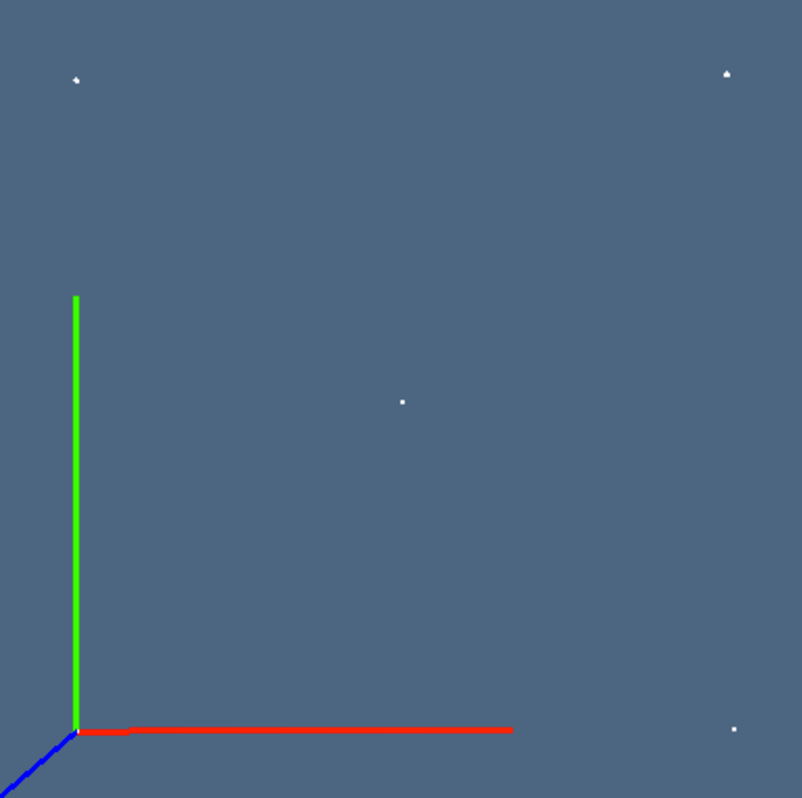
\includegraphics[height=0.245\linewidth,width=0.2425\linewidth]{images/lar2psm-01} 
   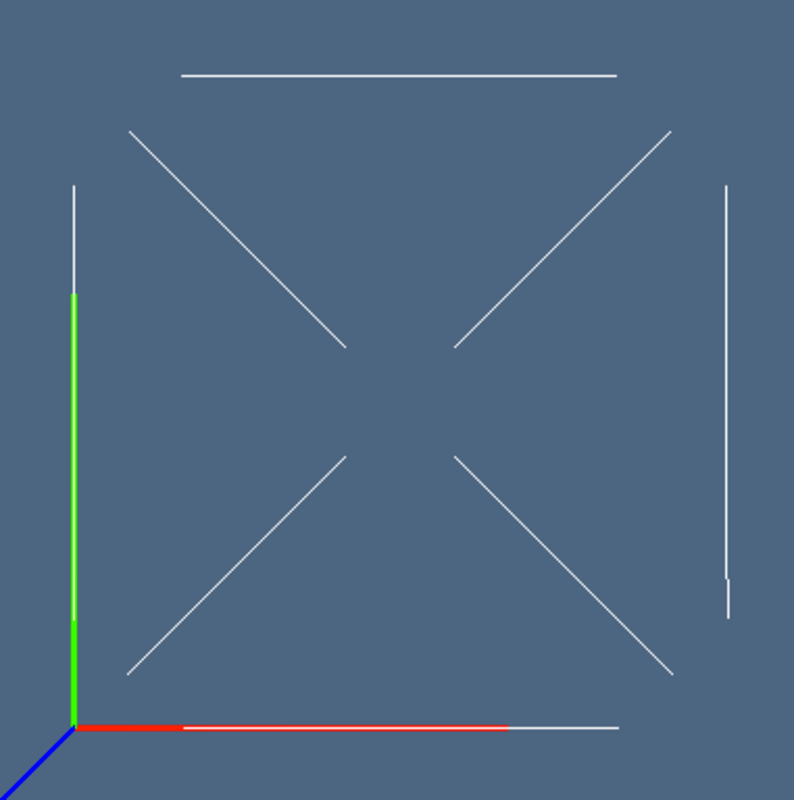
\includegraphics[height=0.245\linewidth,width=0.2425\linewidth]{images/lar2psm-02} 
   
\includegraphics[height=0.245\linewidth,width=0.2425\linewidth]{images/lar2psm-03} 
   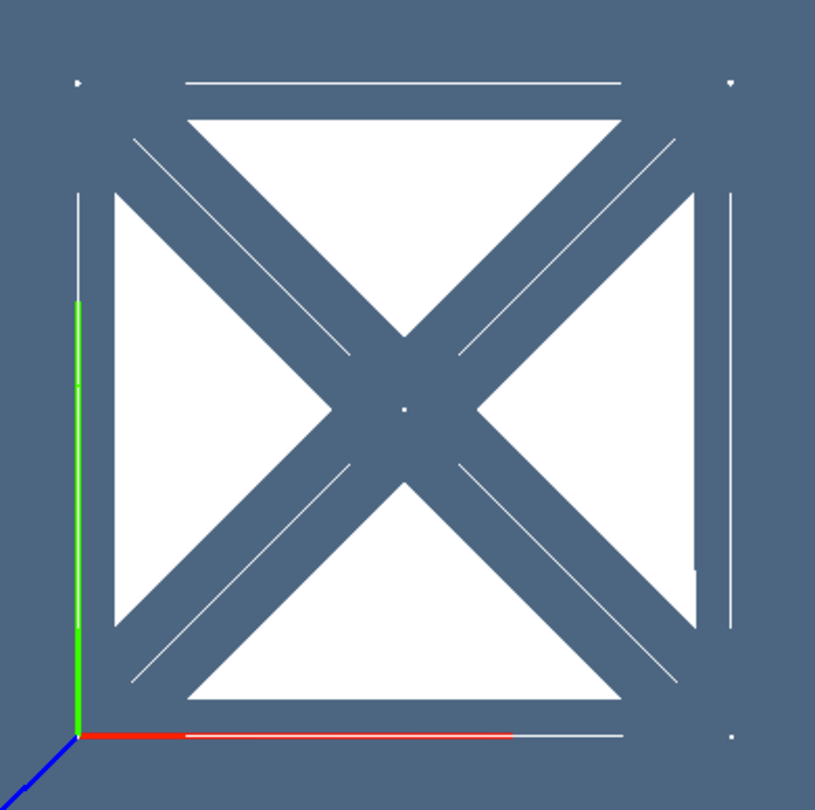
\includegraphics[height=0.245\linewidth,width=0.2425\linewidth]{images/lar2psm-04} 
   \caption{Images of the skeletons of a small simplicial complex.}
   \label{fig:lar2psm-01}
\end{figure}

\subsection{Testing convex combination of vectors}

%------------------------------------------------------------------
@d \texttt{CCOMB} unit tests
@{assert( CCOMB([]) == [] )
assert( CCOMB([[0,1]]) == [0.0, 1.0] )
assert( CCOMB([[0,1],[1,0]]) == [0.5, 0.5] )
assert( CCOMB([[1,0,0],[0,1,0],[0,0,1]]) == [1./3,1./3,1./3])

import random
vects = [[random.random() for i in range(3)] for k in range(4)]
assert( CCOMB([VECTSUM(vects)]) == \
        (sp.array(CCOMB(vects)) * len(vects)).tolist() )
@}
%------------------------------------------------------------------
%@-node:paoluzzi.20131122061759.1684:Unit tests
%@-others
%@nonl
%@-node:paoluzzi.20131121082536.1677:body
%@-others

\bibliographystyle{amsalpha}
\bibliography{lar2psm}

\end{document}
%@-node:paoluzzi.20131121082536.1675:larcc template
%@-others
%@nonl
%@-node:paoluzzi.20131121082536.1674:@shadow ../Documents/dev/test/larcc/src/tex/lar2psm.tex
%@-leo
